\chapter{Planificación}
\label{chap:planification}

\lettrine{U}{n}a vez comentada la metodología a usar, discutiremos cómo se llevó a cabo la planificación de nuestro proyecto. A continuación, presentaremos y analizaremos las diferentes iteraciones que conformaron dicha planificación.

\section{Iteración 1 : Investigación y Preparación Inicial}
\label{chap:investigPlan}

En esta primera iteración partimos desde cero, aún no tenemos nada construido. Esta etapa tuvo una duración de una semana, del 9 al 16 de mayo de 2023.

Primero se realizaron búsquedas de publicaciones sobre la detección de árboles en nubes de puntos. Durante esta fase, nos encontramos con la publicación \cite{rs15061619}, de la cual obtuvimos la idea de utilizar máximos como un enfoque inicial. También destacamos la publicación de \textit{Forest Ecosystems} \cite{ZHANG2023100088}, de la cual tomamos la idea de utilizar las secciones del tronco. Además, en paralelo, comenzamos la búsqueda de repositorios de nubes de puntos. En esta búsqueda tuvimos en cuenta la densidad de puntos, ya que era fundamental poder identificar el tronco ya que en densidades bajas no se pueden ver. Finalmente, después de considerar varias opciones optamos por utilizar el repositorio de Luxemburgo.


Después de informarnos y revisar las aproximaciones ya existentes procedimos a realizar pruebas con la herramienta \textit{WhiteBox Tools} para evaluar diferentes algoritmos destinados a la modificación de nubes de puntos, tales como la eliminación del suelo o la reducción de ruido. Una vez completada esta iteración, concluyó con una reunión con los tutores durante la cual se discutió la información obtenida y se propusieron nuevos objetivos para la próxima iteración.

\section{Iteración 2 : Preparación del entorno de Desarrollo}
En esta segunda fase se comenzó a buscar el entorno y los lenguajes que se utilizarían para desarrollar el trabajo. Durante esta etapa se comenzó barajando la opción de usar el lenguaje \textit{Rust} debido a su gran eficiencia. El problema radica en que aprender este lenguaje en poco tiempo es algo complejo y las bibliotecas disponibles para el procesamiento de nubes de puntos son escasas y tienen poca documentación, por lo que esta opción se descartó.

La otra opción que se barajó fue \textit{Python}. Dado que es un lenguaje más extendido en el mundo del procesamiento de datos y lleva más tiempo en el mercado, ofrece una amplia variedad de herramientas tanto para modificar como para visualizar nubes de puntos. La mayor desventaja de este enfoque es que es un lenguaje de muy alto nivel que, en términos de rendimiento, puede ser el doble de lento a \textit{Rust}. Para solucionarlo inconveniente, existen bibliotecas que permiten llamar a funciones escritas en otro lenguaje, como \textit{C++}, desde nuestro código de \textit{Python}. Un ejemplo de esto es PDAL, que nos permite utilizar el pipeline de procesamiento de nubes de puntos escrito en \textit{C++} desde \textit{Python} o \textit{Conda}. Finalmente, esta fue la opción por la que se optó. Informamos a los tutores de esta decisión y procedimos a la instalación de \textit{Conda} para utilizar PDAL. Esta tarea abarcó desde el 16 de mayo al 23 de mayo de 2023.


\section{Iteración 3 : Desarrollo de una primera versión}
En esta Iteración se procedió a desarrollar una primera versión capaz de convertir la nube de puntos 3d en un matriz 2d que represente la altura de cada punto y a partir de esta matriz obtener los máximos que nos servirán como un punto de partida en la detección.
La primera tarea será convertir ese conjunto de datos 3D en una matriz 2D. Una vez con esta matriz procederemos a buscar los máximos locales dentro de un umbral de vecindad. Esta tarea tomo desde el 23 de mayo hasta el 6 de junio, para terminarla se reunió con los tutores se les presento las nuevas funcionalidades y se propusieron mejoras para una próxima Iteración. 

\section{Iteración 4 : Desarrollo de una  usando Estratos }
En esta fase se desarrollara el algoritmo que comentamos en la sección \ref{chap:Deteccion}. Partiremos de los máximos locales obtenidos previamente para buscar en ellos características que puedan confirmar que es un árbol. En nuestro caso se optó por coger los puntos dentro de una sección cilíndrica con centro en el máximo y radio un parámetro que configuraremos en el código, y partiendo de esos puntos usar técnicas como RANSAC o obtener los centroides de diferentes secciones para determinar si es un árbol o no. A mayores de esto para esta parte de análisis de características se le pasará la nube de puntos con alturas normalizadas y sin suelo, esto lo obtendremos gracias al pipeline de PDAL.

Lo último que se realizó en esta iteración fue que se seleccionaron unos tiles de prueba y se les asignó un clasificación con la localización de los puntos, para hacer esta tarea se desarrolló una pequeña utilidad que guarde los puntos que nosotros marcamos manualmente como árboles en un \textit{CSV}. A partir de estos tiles podremos ir obteniendo unas primeras métricas para ver que tan preciso es nuestro sistema. Esta tarea abarca desde el 7 de junio al 2 de julio.

\section{Iteración 5 : Mejora del Sistema de Centroides}
Anteriormente se creó un sistema para obtener el centroide de diferentes secciones del estrato y comprobar la linealidad, si el valor obtenido era mayor de cierto umbral se clasificaba ese punto como un árbol. En esta iteración se planteo y desarrolló un sistema para que en cada sección se aplique un algoritmo de clustering y obtener el centroide de cada cluster.Esto se decidió hacer así por que previamente la aparición de ramas podaría dar resultado a un falso negativo. Con este nuevo sistema tendremos un árbol con todos los centroides y al recorrer todas las secciones buscaremos en esa estructura de datos el mejor conjunto de centroides, esto lo veremos de manera más detallada en el capitulo \ref{chap:Deteccion}.

A mayores de esto se comenzó a realizar la memoria, en concreto la parte relacionada con el algoritmo comentado previamente.
La realización de esta iteración comenzó el 3 de julio y termino el 17 de ese mismo mes.

\section{Iteración 6 : Pruebas y análisis de los test}
Una vez con el sistema desarrollado se paso a la obtención de los tiles y su preparación para realizar pruebas. Se eligieron solo tiles de Luxemburgo y de diferentes zonas forestales con diferentes tipos de árboles. Sobre estes se realizaron pruebas y se ejecutaron los algoritmos, con los resultados obtenidos se guardaron y se analizaron posteriormente para incluir los resultados obtenidos en la memoria. Esta tarea comenzó el 17 de julio y terminó el 23 de julio.

\section{Iteración 7 : Realización de la Memoria}

En esta última fase con toda la información obtenida a lo largo del desarrollo del proyecto se realizó el desarrollo de la memoria. Se crearon grafismos y diagramas con el fin de que los lectores entiendan mejor el funcionamiento. Para la realización del diagrama de gantt para mostrar la planificación de la memoria se opto por usar la herramienta de código abierto \textit{Mermaid.js} que nos permite la creación de estes mediante código y css. Esta última iteración comenzó el 23 de julio hasta el 10 de septiembre.


\section{Costes}
Una vez con la planificación hecha realizaremos una estimación de los costes de este proyecto. Primero establecemos el coste de los recursos humanos.El coste por hora de un desarrollador junior son aproximadamente 9€/h \cite{saljun} y el coste promedio de dos profesores doctorados por hora es de 18€/h \cite{saldoc}. El tiempo total lo obtendremos de la planificación y suponemos que se trabajan 3 horas al día y las reuniones con los tutores son de 2h. El coste total lo vemos en la tabla \ref{tabcospes}

\begin{table}[hp!]
   \centering
  \rowcolors{2}{white}{udcgray!25}
  \begin{tabular}{c|c|c|c}
  \rowcolor{udcpink!25}
  \textbf{Nombre del Recurso} & \textbf{Coste por hora} & \textbf{Horas Trabajadas} & \textbf{Total}\\\hline
  
  Programador Junior & 9 €/h & 420 h & 3780 € \\
  Tutor 1 & 18 €/h & 18 h & 324 € \\
  Tutor 2 & 18 €/h & 18 h & 324 €  \\
  \textbf{Total}  & & & \textbf{4428 €}\\

  \end{tabular}

  \caption{Tabla con el desglose de los costes humanos}
  \label{tabcospes}


\end{table}

  Ahora nombraremos los costes materiales, en esta parte contaremos tanto los recursos físicos como el ordenador como el coste de las licencias del software usado. Primero empezaremos por el ordenador, estos tienen un ciclo de vida de entre 6 a 10 años y su costo fue de 900 €, si el proyecto duró 4 meses y la vida media la definimos en 7 años el coste por mes sería de sobre 11 € al mes. Para el desarrollo se uso el IDE \textit{Pycharm} de la empresa \textit{JetBrains}  que tiene un coste de 24.99 € al mes \cite{costjet}.

\begin{table}[hp!]
   \centering
  \rowcolors{2}{white}{udcgray!25}
  \begin{tabular}{c|c|c|c}
  \rowcolor{udcpink!25}
  \textbf{Nombre del Recurso} & \textbf{Coste Mensual} & \textbf{Meses de Uso} & \textbf{Total}\\\hline
  
  Ordenador & 11 €/mes & 4 meses & 44 € \\
  Licencia Pycharm & 24.99 €/mes & 4 meses & 99.96 € \\
  \textbf{Total}  & & & \textbf{143.96 €} \\
  \end{tabular}

  \caption{Tabla con el desglose de los costes materiales}
  \label{tabcospes}
\end{table}

Con todo esto en la figura \ref{tabcostot} vemos el coste total del proyecto.

\begin{table}[hp!]
   \centering
  \rowcolors{2}{white}{udcgray!25}
  \begin{tabular}{c|c}
  \rowcolor{udcpink!25}
  \textbf{Nombre del Recurso} & \textbf{Coste} \\\hline
  
  Costes Humanos & 4428 € \\
  Costes Materiales & 143.96 €  \\
  \textbf{Total}  &  \textbf{4571.96 €} \\
  \end{tabular}

  \caption{Tabla con el coste total}
  \label{tabcostot}
\end{table}


\begin{figure}[h]
\centering
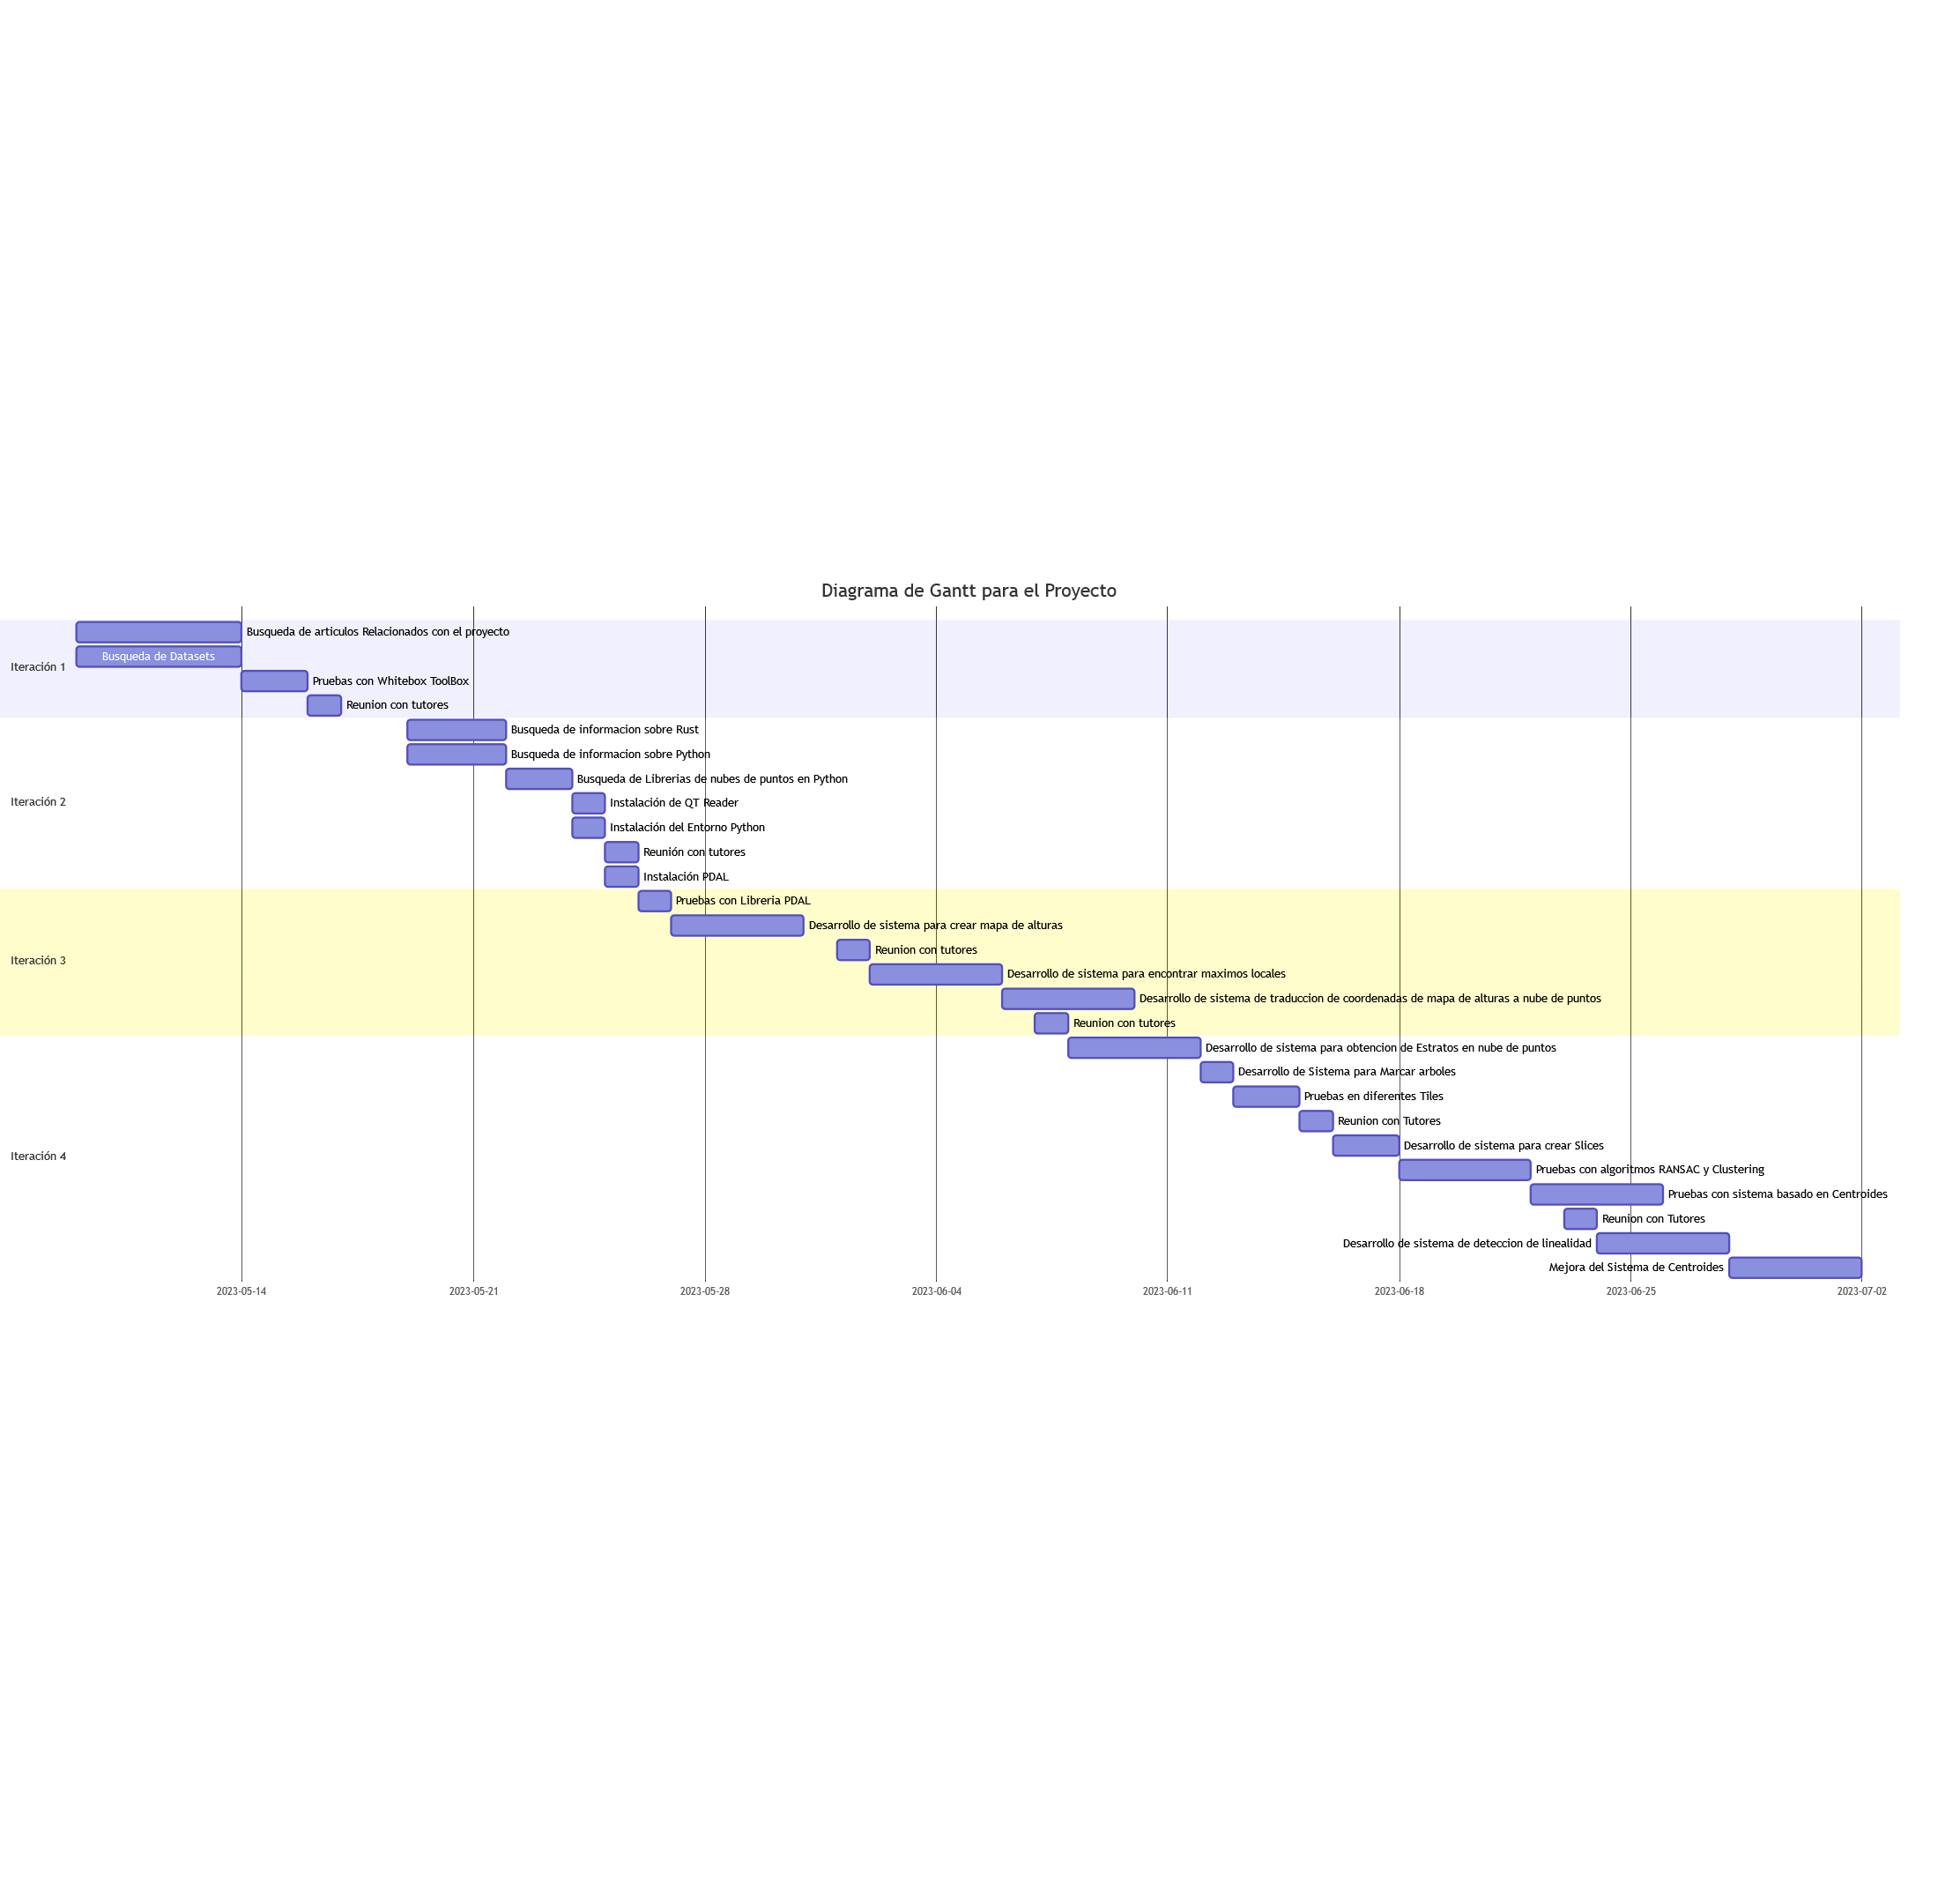
\includegraphics[width=15cm]{imaxes/gantt1.png}
\label{fig:pointnetc}
\caption{Primeras 4 iteraciones del Diagrama de Gantt}
\end{figure}

\begin{figure}[h]
\centering
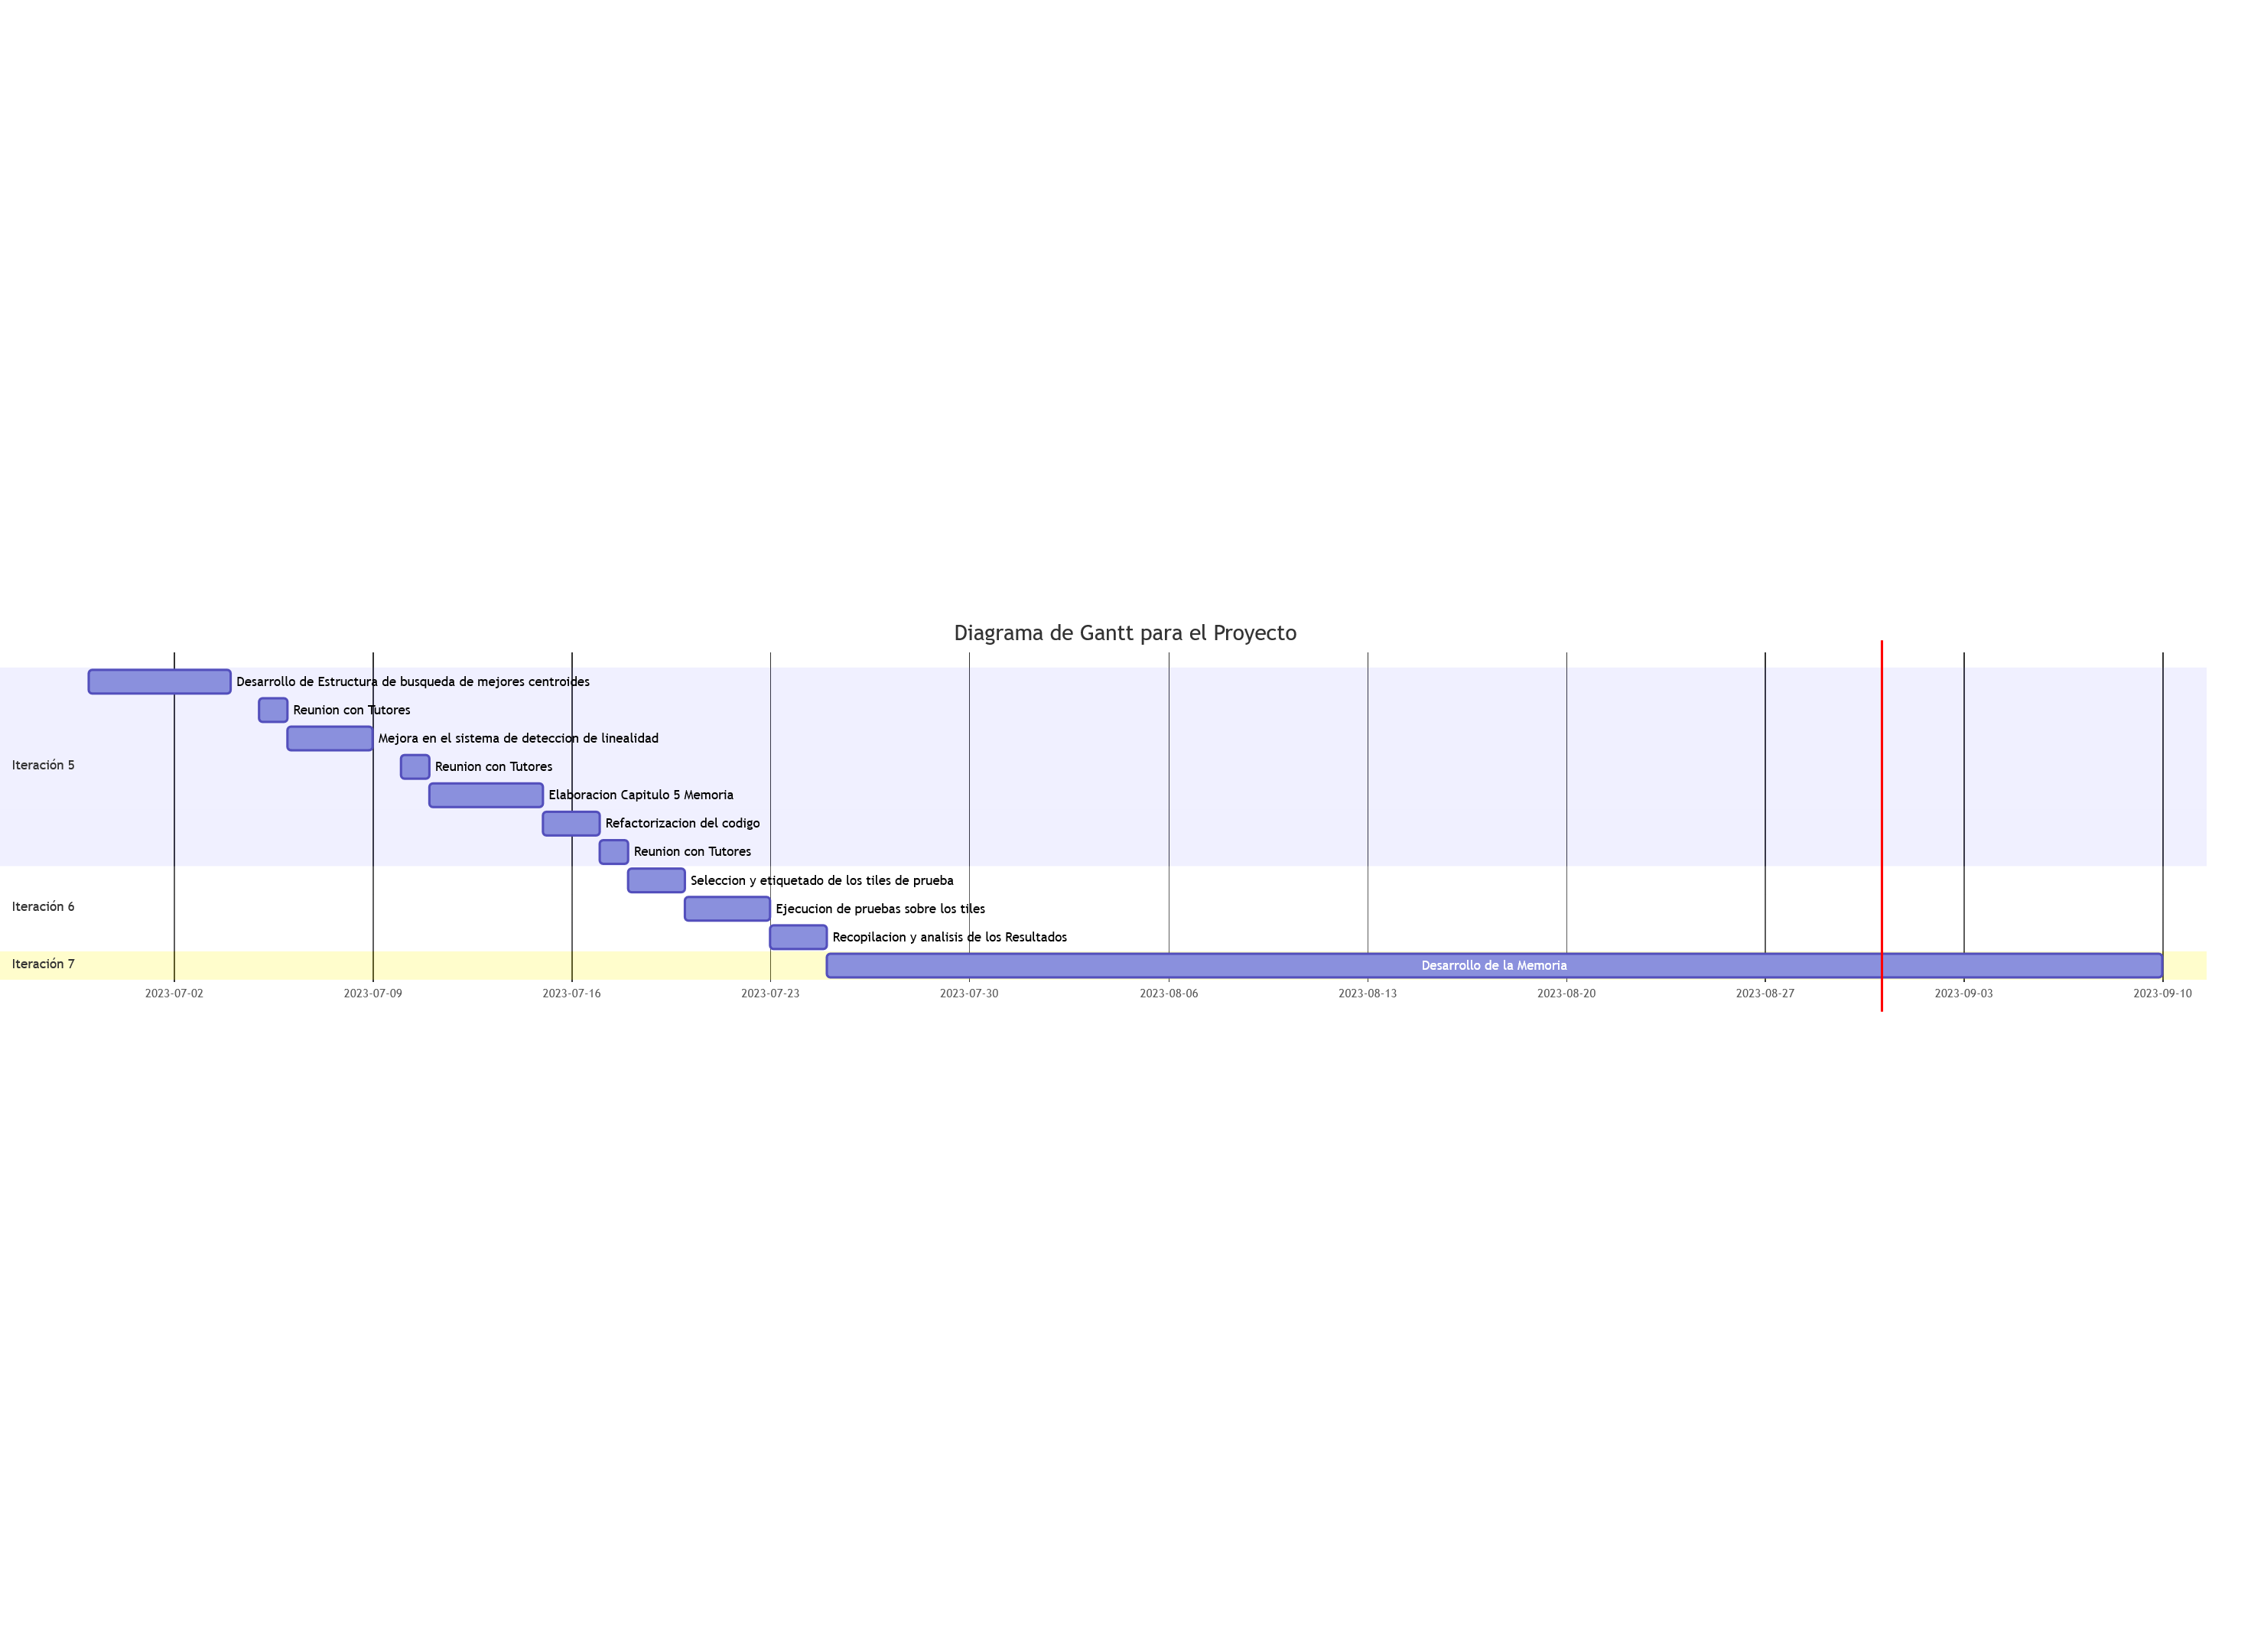
\includegraphics[width=15cm]{imaxes/gantt2.png}
\label{fig:pointnetc}
\caption{Últimas iteraciones del Diagrama de Gantt}
\end{figure}

